\documentclass[12pt]{report}
\usepackage[utf8]{inputenc}
\usepackage[russian]{babel}
%\usepackage[14pt]{extsizes}
\usepackage{listings}
\usepackage{graphicx}
\usepackage{amsmath,amsfonts,amssymb,amsthm,mathtools} 
\usepackage{pgfplots}
\usepackage{filecontents}
\usepackage{indentfirst}
\usepackage{eucal}
\usepackage{float}
\usepackage{amsmath}
\usepackage{enumitem}
\frenchspacing

\usepackage{indentfirst} % Красная строка


%\usetikzlibrary{datavisualization}
%\usetikzlibrary{datavisualization.formats.functions}

\usepackage{amsmath}


% Для листинга кода:
\lstset{ %
	language=haskell,                 % выбор языка для подсветки (здесь это С)
	basicstyle=\small\sffamily, % размер и начертание шрифта для подсветки кода
	numbers=left,               % где поставить нумерацию строк (слева\справа)
	numberstyle=\tiny,           % размер шрифта для номеров строк
	stepnumber=1,                   % размер шага между двумя номерами строк
	numbersep=5pt,                % как далеко отстоят номера строк от подсвечиваемого кода
	showspaces=false,            % показывать или нет пробелы специальными отступами
	showstringspaces=false,      % показывать или нет пробелы в строках
	showtabs=false,             % показывать или нет табуляцию в строках
	frame=single,              % рисовать рамку вокруг кода
	tabsize=2,                 % размер табуляции по умолчанию равен 2 пробелам
	captionpos=t,              % позиция заголовка вверху [t] или внизу [b] 
	breaklines=true,           % автоматически переносить строки (да\нет)
	breakatwhitespace=false, % переносить строки только если есть пробел
	escapeinside={\#*}{*)}   % если нужно добавить комментарии в коде
}

\linespread{1.5}
\usepackage[left=2cm,right=2cm, top=2cm,bottom=2cm,bindingoffset=0cm]{geometry}
% Для измененных титулов глав:
\usepackage{titlesec, blindtext, color} % подключаем нужные пакеты
\definecolor{gray75}{gray}{0.75} % определяем цвет
\newcommand{\hsp}{\hspace{20pt}} % длина линии в 20pt
% titleformat определяет стиль
\titleformat{\chapter}[hang]{\Huge\bfseries}{\thechapter\hsp\textcolor{gray75}{|}\hsp}{0pt}{\Huge\bfseries}


% plot
\usepackage{pgfplots}
\usepackage{filecontents}
\usetikzlibrary{datavisualization}
\usetikzlibrary{datavisualization.formats.functions}

\begin{document}
	%\def\chaptername{} % убирает "Глава"
	\thispagestyle{empty}
	\begin{titlepage}
		\noindent \begin{minipage}{0.15\textwidth}
			
\includegraphics[width=\linewidth]{b_logo}
		\end{minipage}
		\noindent\begin{minipage}{0.9\textwidth}\centering
			\textbf{Министерство науки и высшего образования Российской Федерации}\\
			\textbf{Федеральное государственное бюджетное образовательное учреждение высшего образования}\\
			\textbf{~~~«Московский государственный технический университет имени Н.Э.~Баумана}\\
			\textbf{(национальный исследовательский университет)»}\\
			\textbf{(МГТУ им. Н.Э.~Баумана)}
		\end{minipage}
		
		\noindent\rule{18cm}{3pt}
		\newline\newline
		\noindent ФАКУЛЬТЕТ $\underline{\text{«Информатика и системы управления»}}$ \newline\newline
		\noindent КАФЕДРА $\underline{\text{«Программное обеспечение ЭВМ и информационные технологии»}}$\newline\newline\newline
		
		
		\begin{center}
			\noindent\begin{minipage}{1.3\textwidth}\centering
				\Large\textbf{  Отчёт по лабораторной работе №6}\newline
				\textbf{по дисциплине "Анализ алгоритмов"}\newline\newline
			\end{minipage}
		\end{center}
		
		\noindent\textbf{Тема} $\underline{\text{Муравьиный алгоритм и метод полного перебора для решения задачи коммивояжёра}}$\newline
		\noindent\textbf{Студент} $\underline{\text{Романов А.В.}}$\newline
		\noindent\textbf{Группа} $\underline{\text{ИУ7-53Б}}$\newline
		\noindent\textbf{Преподаватели} $\underline{\text{Волкова Л.Л., Строганов Ю.В.}}$\newline\newline\newline\newline
		
		\begin{center}
			\vfill
			Москва~---~\the\year
			~г.
		\end{center}
	\end{titlepage}
	
	
	\tableofcontents
	
\newpage
\chapter*{Введение}
\addcontentsline{toc}{chapter}{Введение}
	
Муравьиный алгоритм -- один из эффективных полиномиальных алгоритмов для нахождения приближённых решений задачи коммивояжёра, а также решения аналогичных задач поиска маршрутов на графах. Суть подхода заключается в анализе и использовании модели поведения муравьёв, ищущих пути от колонии к источнику питания, и представляет собой метаэвристическую оптимизацию.
	
\section*{Цель лабораторной работы}
	
Целью данной лабораторной работы является изучение муравьиного алгоритма и приобретение навыков параметризации методов на примере муравьиного алгоритма.
	
\section*{Задачи лабораторной работы}
	
В рамках выполнения работы необходимо решить следующие задачи:
	
\begin{itemize}
	\item решить задачу коммивояжера при помощи алгоритма полного перебора и муравьиного алгоритма;
	\item замерить и сравнить время выполнения алгоритмов;
	\item протестировать муравьиный алгоритм на разных переменных;
	\item сделать выводы на основе проделанной работы.
\end{itemize}
	
\chapter{Аналитическая часть}
	
В данном разделе представленные теоретические сведения о рассматриваемых алгоритмах.

\section{Полный перебор}

Пронумеруем все города от 1 до $n$. Базовому городу присвоим номер n. Каждый тур по городам однозначно соответствует перестановке целых чисел $1, 2, ..., n-1$.


Задачу коммивояжера можно решить образуя все перестановки первых $n-1$ целых положительных чисел. Для каждой перестановки строится соответствующий тур и вычисляется его стоимость. Обрабатывая таким образом все перестановки, запоминается тур, который к текущему моменту имеет наименьшую стоимость. Если находится тур с более низкой стоимостью, то дальнейшие сравнения производятся с ним.


Сложность алгоритма полного перебора составляет $O(n!)$ \cite{goodman}.
	
\section{Муравьиный алгоритм}

Моделирование поведения муравьев связано с распределением феромона на тропе — ребре графа в задаче коммивояжера. При этом вероятность включения ребра в маршрут отдельного муравья пропорциональна количеству феромона на этом ребре, а количество откладываемого феромона пропорционально длине маршрута. Чем короче маршрут, тем больше феромона будет отложено на его ребрах, следовательно, большее количество муравьев будет включать его в синтез собственных маршрутов. Моделирование такого подхода, использующего только положительную обратную связь, приводит к преждевременной сходимости — большинство муравьев двигается по локально оптимальному маршруту. Избежать, этого можно, моделируя отрицательную обратную связь в виде испарения феромона. При этом если феромон испаряется быстро, то это приводит к потере памяти колонии и забыванию хороших решений, с другой стороны, большое время испарения может привести к получению устойчивого локально оптимального решения. Теперь, с учетом особенностей задачи коммивояжера, мы можем описать локальные правила поведения муравьев при выборе пути.

\begin{itemize}
	\item муравьи имеют собственную «память». Поскольку каждый город может быть посещеи только один раз, у каждого муравья есть список уже посещенных городов --- список запретов. Обозначим через $J_{i,k}$ список городов, которые необходимо посетить муравью $k$, находящемуся в городе $i$;
	\item муравьи обладают «зрением» --- видимость есть эвристическое желание посетить город $j$, если муравей находится в городе $i$. Будем считать, что видимость обратно пропорциональна расстоянию между городами $i$ и $j$ --- $D_{ij}$ 
	\begin{equation}
	\label{eq:vision}
	\eta_{ij} = \frac{1}{D_{ij}}
	\end{equation}
	\item муравьи обладают «обонянием» — они могут улавливать след феромона, подтверждающий желание посетить город $j$ из города $i$, на основании опыта других муравьев. Количество феромона на ребре $(i,j)$ в момент времени $t$ обозначим через $\tau_{ij}(t)$.
\end{itemize}

На этом  основании мы можем сформулировать вероятностно-пропорциональное правило \ref{eq:rule}, определяющее вероятность перехода $k$-ого муравья из города $i$ в город $j$:

\begin{equation}
	\label{eq:rule}
	\begin{cases}
	P_{i,j,k}(t) = \frac{[\tau_{ij}(t)]^\alpha*[\eta_{ij}]^\beta}{\sum_{l\in J_{i,k}}^{}[\tau_{il}(t)]^\alpha * [\eta_{il}]^\beta}, & j \in J_{i,k};\\
	P_{i,j,k}(t) = 0, & j \notin J_{i,k},
	\end{cases}
\end{equation}


где $\alpha, \beta$ — параметры, задающие веса следа феромона, при $\alpha=0$ алгоритм вырождается до жадного алгоритма (будет выбран ближайший город). Заметим, что
выбор города является вероятностным, правило \ref{eq:rule} лишь определяет ширину
зоны города $j$; в общую зону всех городов $J_{i,k}$;, бросается случайное число, которое и определяет выбор муравья. Правило \ref{eq:rule} не изменяется в ходе алгоритма, но у двух разных муравьев значение вероятности перехода будут отличаться, т. к. они имеют разный список разрешенных городов.

Пройдя ребро $(i,j)$, муравей откладывает на нем некоторое количество феромона, которое должно быть связано с оптимальностью сделанного выбора. Пусть $T_k(t)$ есть маршрут, пройденный муравьем $k$ к моменту времени t, а $L_k(t)$ --- длина этого маршрута. Пусть также $Q$ --- параметр, имеющий значение порядка длины оптимального пути. Тогда откладываемое количество феромона может быть задано в виде:

\begin{equation}
	\label{eq:pheromone_drop}
	P_{i,j,k}(t) =
	\begin{cases}
	\frac{Q}{L_{k}(t)}, & (i,j) \in T_{k}(t);\\
	0, & (i,j) \notin T_{k}(t).
	\end{cases}
\end{equation}

Правила внешней среды определяют, в первую очередь, испарение феромона. Пусть $\rho \in [0,1]$ есть коэффициент испарения, тогда правило испарения имеет вид

\begin{equation}
	\label{eq:pheromone_evaporation}
	\tau_{ij}(t+1) = (1 - \rho) * \tau_{ij}(t) + \Delta\tau_{ij}(t); \Delta\tau_{ij}(t) = \sum_{k = 1}^{m} \Delta\tau_{ij,k}(t); 
	\end{equation}

где $m$ — количество муравьев в колонии.

В начале алгоритма количество феромона на ребрах принимается равным
небольшому положительному числу. Общее количество муравьев остается постоянным и равным количеству городов, каждый муравей начинает маршрут из своего города. 

Сложность алгоритма: $O(t_{max} * max(m, n^2))$, где $t_{max}$ --- время жизни колонии, $m$ --- количество муравьев в колонии, $n$ --- размер графа \cite{ulyanov}.

\section*{Вывод}
В данном разделе были рассмотренны особенности алгоритмов решения задачи коммивояжёра.
	
\chapter{Конструкторская часть}
	
В данном разделе представлены схемы рассматриваемых алгоритмов.
	
\section{Разработка алгоритмов}
	
На рисунках \ref{fig:bruteforce} - \ref{fig:ant} приведены схемы алгоритмов решения задачи коммивояжера.
	
\begin{figure}[H]
		\centering
		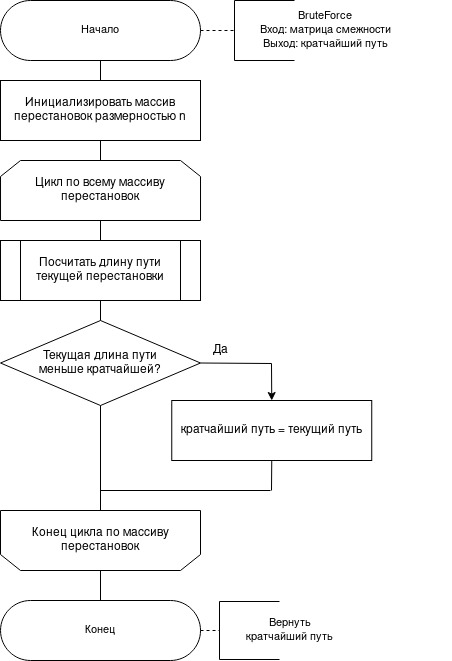
\includegraphics[scale=0.62]{bruteforce.jpg}
		\caption{Схема алгоритма полного перебора.}
		\label{fig:bruteforce}
\end{figure}

\begin{figure}[H]
		\centering
		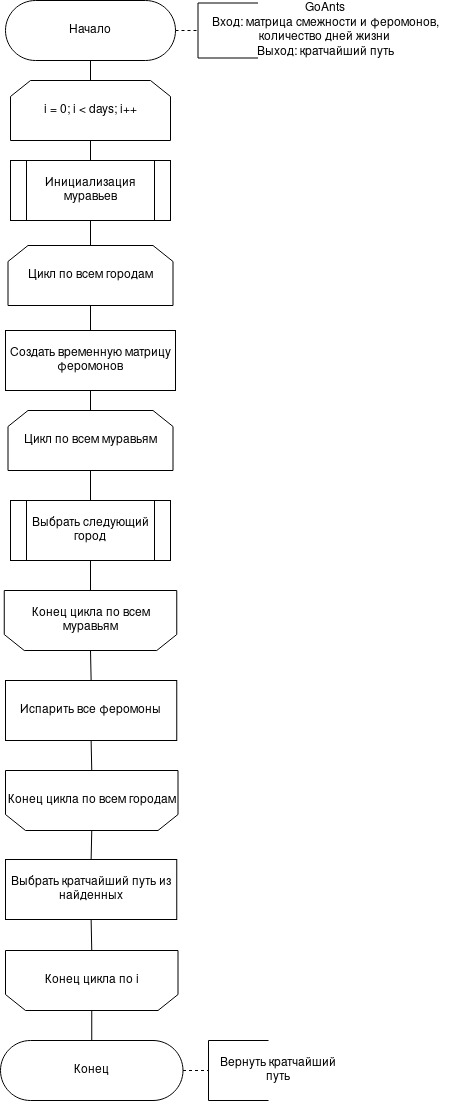
\includegraphics[scale=0.6]{ant.jpg}
		\caption{Схема муравьиного алгоритма.}
		\label{fig:ant}
\end{figure}
	
\section{Автоматическая параметризация}

Автоматическая параметризация выполняет проверку дней $= [1..v]$ (где $v$ --- размер графа), $\alpha$ = [0..1], $\rho = [0..1]$ независимо друг от друга.


Алгоритм запускается три раза и минимальное значение сравнивается с эталонным. Затем на экран выводятся параметры и сравниваются с эталонными значениями.
	
\section*{Вывод}
	
На основе теоретических данных, полученных аз аналитического раздела, были построенны схемы алгоритмов для решения задачи коммивояжёра.
	
\chapter{Технологическая часть}
	
В данном разделе приведены средства реализации и листинги кода.
	
\section{Требование к ПО}
	
К программе предъявляется ряд требований:
	
\begin{itemize}
	\item на вход подается матрица смежности, со значениями не более чем максимальное целое число деленное пополам;
	\item на выходе -- кратчайший путь.
\end{itemize}
	
\section{Средства реализации}
	
Для реализации ПО я выбрал язык программирования Golang \cite{golang}. Данный выбор обусловлен моим желанием расширить свои знания в области применения данного языка программирования.
	
\section{Реализация алгоритмов}

В листингах 3.1 - 3.2 представлены листинги алгоритмов решения задачи коммивояжёра.
	
\begin{lstlisting}[label=some-code,caption=Алгоритм полного перебора, language=go]
func BruteForce(graph [][]int) []int {
	path := make([]int, 0)
	shortest := make([]int, len(graph))
	
	for r := 0; r < len(graph); r++ {
		routes := make([][]int, 0)
		calculateRoutes(r, graph, path, &routes)
	
		minSum := int(MaxInt)
	
		for i := 0; i < len(routes); i++ {
			curr := 0
				for j := 0; j < len(routes[i])-1; j++ {
					curr += graph[routes[i][j]][routes[i][j+1]]
				}
	
				if curr < minSum {
					minSum = curr
				}
			}

		shortest[r] = minSum
	}

	return shortest
}

func calculateRoutes(position int, graph [][]int, path []int, routes *[][]int) {
	path = append(path, position)
	
	if len(path) < len(graph) {
		for i := 0; i < len(graph); i++ {
			if !pathContains(path, i) {
				calculateRoutes(i, graph, path, routes)
			}
		}
	} else {
		*routes = append(*routes, path)
	}
}

func pathContains(path []int, value int) bool {
	for i := 0; i < len(path); i++ {
		if path[i] == value {
			return true
		}
	}
	
	return false
}
\end{lstlisting}
	
\begin{lstlisting}[label=some-code,caption=Муравьиный алгоритм, language=go]
func GoAnts(colony *Colony, days int) []int {
	shortest := make([]int, len(colony.graph))
	
	for i := 0; i < days; i++ {
		for j := 0; j < len(colony.graph); j++ {
			ant := colony.createAnt(j)
			ant.startMove()
			current := ant.distance()
	
			if (current < shortest[j]) || (0 == shortest[j]) {
				shortest[j] = current
			}
		}
	}
	
	return shortest
}

func CreateColony(graph [][]int) *Colony {
	colony := new(Colony)
	colony.graph = graph
	colony.pheromon = make([][]float64, len(colony.graph))
	
	for i := 0; i < len(colony.graph); i++ {
		colony.pheromon[i] = make([]float64, len(colony.graph[i]))
		for j := 0; j < len(colony.pheromon[i]); j++ {
			colony.pheromon[i][j] = pheromonCoef
		}
	}
	
	return colony
}


func (colony *Colony) createAnt(position int) *Ant {
	ant := new(Ant)
	ant.colony = colony
	ant.visited = make([][]int, len(colony.graph))
	
	for i := 0; i < len(colony.graph); i++ {
		ant.visited[i] = make([]int, len(colony.graph))
		
		for j := 0; j < len(colony.graph[i]); j++ {
			ant.visited[i][j] = colony.graph[i][j]
		}
	}
	
	ant.pos = position
	ant.path = make([][]bool, len(colony.graph))
	
	for i := 0; i < len(colony.graph); i++ {
		ant.path[i] = make([]bool, len(colony.graph))
	}
	
	return ant
}

func (ant *Ant) makeMove(j int) {
	for i := range ant.visited {
		ant.visited[i][ant.pos] = 0
	}
	
	ant.path[ant.pos][j] = true
	ant.pos = j
}

func (ant *Ant) startMove() {
	way := MaxInt
	
	for cond := true; cond; cond = (way != MinInt) {
		way = chooseWay(ant.getProbability())
	
		if MinInt != way {
			ant.makeMove(way)
			ant.updatePheromon()
		}
	}
}

func (ant *Ant) getProbability() []float64 {
	probability := make([]float64, 0)
	sum := float64(0)
	
	for i, j := range ant.visited[ant.pos] {
		if 0 != j {
			d := math.Pow(ant.colony.pheromon[ant.pos][i], betta) * math.Pow((float64(1)/float64(j)), alpha)
			probability = append(probability, d)
			sum += d
		} else {
			probability = append(probability, 0)
		}
	}
	
	for _, val := range probability {
		val = val / sum
	}
	
	return probability
}

func chooseWay(path []float64) int {
	sum := float64(0)
	
	for _, j := range path {
		sum += j
	}
	
	random := rand.New(rand.NewSource(time.Now().UnixNano())).Float64() * sum
	sum = 0
	
	for i, j := range path {
		if random < sum+j && random > sum {
			return i
	}
	
		sum += j
	}
	
	return MinInt
}

func (ant *Ant) updatePheromon() {
	delta := float64(0)
	
	for r := 0; r < len(ant.colony.pheromon); r++ {
		for i, j := range ant.colony.pheromon[r] {
	
			if 0 != ant.colony.graph[r][i] {
				delta = 0
				if ant.path[r][i] {
					delta = q / float64(ant.colony.graph[r][i])
				}
	
				ant.colony.pheromon[r][i] = (1 - p) * (float64(j) + delta)
			}
	
			if ant.colony.pheromon[r][i] <= 0 {
				ant.colony.pheromon[r][i] = 0.1
			}
		}
	}
}

func (ant *Ant) distance() int {
	distance := 0

	for i, j := range ant.path {
		for k, sign := range j {
			if sign {
				distance += ant.colony.graph[i][k]
			}
		}
	}
	
	return distance
}

\end{lstlisting}

\section{Тестовые данные}

В таблице \ref{tab:test} приведены тестовые данные. Все тесты были пройденны успешно.

\begin{table}[h!]

	\begin{center}

		\begin{tabular}{c@{\hspace{7mm}}c@{\hspace{7mm}}c@{\hspace{7mm}}c@{\hspace{7mm}}c@{\hspace{7mm}}c@{\hspace{7mm}}}

			\hline

			Матрица смежности & Ожидаемый результат & Полученный результат\\ \hline

			\vspace{4mm}		

			$\begin{bmatrix}

			0 & 3 & 1 & 6 & 8\\

			3 & 0 & 4 & 1 & 0\\

			1 & 4 & 0 & 5 & 0\\

			6 & 1 & 5 & 6 & 1\\

			8 & 0 & 0 & 1 & 0

			\end{bmatrix}$ & 15 & 15\\

			$\begin{bmatrix}

			0 & 10 & 15 & 20\\

			10 & 0 & 35 & 25\\

			15 & 35 & 0 & 30\\

			20 & 25 & 30 & 0

			\end{bmatrix}$ & 80 & 80 \\

			
		\end{tabular}

	\end{center}

	\caption{\label{tab:test} Тестирование алгоритмов.}

\end{table}
	
\section*{Вывод}
	
В данном разделе были разработаны и протестированны алгоритмы решения задачи коммивояжёра.
	
\chapter{Исследовательская часть}
	
В данном разделе приведен анализ характеристик разработанного ПО.

\section{Технические характеристики}
	
Ниже приведены технические характеристики устройства, на котором было проведено тестирование ПО:
	
\begin{itemize}
	\item Операционная система: Debian \cite{debian} Linux \cite{linux} 11 <<bullseye>> 64-bit.
	\item Оперативная память: 12 GB.
	\item Процессор: Intel(R) Core(TM) i5-3550 CPU @ 3.30GHz \cite{i5}.	
\end{itemize}
	
\section{Время выполнения алгоритмов}
	
Время выполнения алгоритма замерялось с помощью встроенной функции time.Now() из библиотеки Time \cite{time}. Полученные результаты приведены в таблице \ref{tab:timing}.



\begin{table}[H]

	\begin{center}

		\begin{tabular}{|c|c|c|}

			\hline

			Размер графа & Полный перебор & Муравьиный алгоритм \\

			\hline
			3 & 1 490 & 81 200 \\ 
			5 & 2 500 & 143 100 \\
			7 & 43 220 & 698 700 \\ 
			9 & 2 240 905 & 1 290 500 \\
			11 & 31 470 700 & 2 100 340 \\
			\hline

		\end{tabular}

	\end{center}

	\caption{Сравнение времени исполнения алгоритмов решения задачи коммивояжера.}

	\label{tab:timing}

\end{table}

\section{Автоматическая параметризация}

В таблице \ref{tab:v5} приведена выборка результатов параметризации для матрицы смежности размером 10х10. Количество дней принято равным 100. Полным перебором был посчитан оптимальный путь -- он составил 130.

\begin{table}[H]

	\caption{Выборка из параметризации для матрицы размером $10x10$.}
	\label{tab:v5}
	\begin{center}

		\begin{tabular}{|c@{\hspace{7mm}}|c@{\hspace{7mm}}|c@{\hspace{7mm}}|c@{\hspace{7mm}}|c@{\hspace{7mm}}|c|}

			\hline
			$\alpha$        & $\beta$      & $\rho$      &Длина  & Разница \\

			\hline

			0    & 1    & 0.0    & 130    & 0     \\
			0    & 1    & 0.3    & 130    & 0     \\
            0    & 1    & 0.5    & 131    & 1     \\
            0    & 1    & 1.0    & 130    & 0     \\
            \hline
            0.1  & 0.9  & 0.0    & 130    & 0     \\
            0.1  & 0.9  & 0.3    & 130    & 0     \\
			0.1  & 0.9  & 0.6    & 131    & 1     \\                    
			0.1  & 0.9  & 1.0    & 130    & 0     \\
			\hline

			0.2  & 0.8  & 0.0    & 130    & 0     \\
			0.2  & 0.8  & 0.3    & 131    & 1     \\
			0.2  & 0.8  & 0.6    & 131    & 1     \\
			0.2  & 0.8  & 1.0    & 130    & 0     \\
			\hline
			0.3  & 0.7  & 0.0  & 131    & 1     \\
			0.3  & 0.7  & 0.4  & 130    & 0     \\
			0.3  & 0.7  & 0.9  & 131    & 1     \\
			0.3  & 0.7  & 1.0  & 130    & 0     \\
			\hline
			0.4  & 0.6  & 0.0  & 130    & 0     \\
			0.4  & 0.6  & 0.4  & 131    & 1     \\
			0.4  & 0.6  & 0.5  & 130    & 0     \\
			0.4  & 0.6  & 1.0  & 130    & 0     \\
			\hline
			0.5  & 0.5  & 0.0  & 130    & 0     \\
			0.5  & 0.5  & 0.3  & 131    & 1     \\
			0.5  & 0.5  & 0.7  & 131    & 1     \\
			0.5  & 0.5  & 1.0  & 130    & 0     \\
			\hline
			0.6  & 0.4  & 0.2  & 136    & 6     \\
			0.6  & 0.4  & 0.6  & 133    & 3     \\
			0.6  & 0.4  & 0.7  & 130    & 0     \\
			0.6  & 0.4  & 0.7  & 130    & 0     \\
			\hline
		\end{tabular}
	\end{center}
\end{table}

\begin{table}[H]
	\begin{center}
\begin{tabular}{|c@{\hspace{7mm}}|c@{\hspace{7mm}}|c@{\hspace{7mm}}|c@{\hspace{7mm}}|c@{\hspace{7mm}}|c|}
		\hline
			$\alpha$        & $\beta$      & $\rho$      &Длина  & Разница \\
			
			\hline
			0.7  & 0.3  & 0.0  & 130    & 0     \\
			0.7  & 0.3  & 0.3  & 134    & 4     \\
			0.7  & 0.3  & 0.6  & 132    & 2     \\
			0.7  & 0.3  & 0.8  & 139    & 9     \\
			\hline
			0.8  & 0.2  & 0.0  & 140    & 10    \\
			0.8  & 0.2  & 0.5  & 134    & 4     \\
			0.8  & 0.2  & 0.7  & 131    & 1     \\
			0.8  & 0.2  & 1.0  & 130    & 0     \\
			\hline
			0.9  & 0.1  & 0.0  & 134    & 4     \\
			0.9  & 0.1  & 0.3  & 132    & 2     \\
			0.9  & 0.1  & 0.5  & 134    & 4     \\
			0.9  & 0.1  & 1.0  & 130    & 0     \\
			\hline
			1.0  & 0.0  & 0.0  & 145    & 25     \\
			1.0  & 0.0  & 0.4  & 133    & 3     \\
			1.0  & 0.0  & 0.7  & 142    & 22     \\
			1.0  & 0.0  & 1.0  & 138    & 8     \\
			\hline
	\end{tabular}

\end{center}

\end{table}

\section*{Вывод}

При небольших размерах графа (от 3 до 7) алгоритм полного перебора выигрывает по времени у муравьиного. Например, при размере графа 5, полный перебор работает быстрее примерно в 57 раз. Однако, при увеличении размера графа (от 9 и выше), ситуация меняется в обратную сторону: муравьиный алгоритм начинает значительно выигрывать по времени у алгоритма полного перебора. На размерах графа 11, муравьиный алгоритм работает в 15 раз быстрее.

Наиболее стабильные результаты автоматической параметризации получаются при наборе $\alpha = 0.1..0.5$, $\beta = 0.1..0.5$, $\rho = $ любое. При таких параметрах полученный результат не отличается более чем на 1 от эталонного, и, в около 75\% (на промежутке $\rho = 0.0..1.0$) случаев полученный результат совпадает с эталонным. Наиболее нестабильные результаты полученны при $\alpha = 1.0$, $\beta = 0.0$, $\rho = $ любое.

\chapter*{Заключение}
\addcontentsline{toc}{chapter}{Заключение}
	
В рамках данной лабораторной работы лабораторной работы была достигнута её цель: изучен муравьиный алгоритм и приобретены навыки параметризации методов на примере муравьиного алгоритма. Также выполнены следующие задачи:
	
\begin{itemize}
	\item реализованны два алгоритма решения задачи коммивояжера;
	\item замерено время выполнения алгоритмов;
	\item муравьиный алгоритм протестирован на разных переменных;
	\item сделаны выводы на основе проделанной работы;
\end{itemize}

Использовать муравьиный алгоритм для решения задачи коммивояжера выгодно (с точки зрения времени выполнения), в сравнении с алгоритмом полного перебора, в случае если в анализируемом графе вершин больше либо равно 9. Так, например, при размере графа 11, муравьиный алгоритм работает быстрее чем алгоритм полного перебора в 15 раз. Стоит отметить, что муравьиный алгоритм не гарантирует что найденный путь будем оптимальным, так как он является эвристическим алгоритмом, в отличии от алгоритма полного перебора.

\addcontentsline{toc}{chapter}{Литература}
\bibliographystyle{utf8gost705u}  % стилевой файл для оформления по ГОСТу
\bibliography{51-biblio}          % имя библиографической базы (bib-файла)
	
\end{document}
